\documentclass[11pt]{article}

\usepackage[margin=1in]{geometry}
\usepackage{amsmath}
\usepackage{amssymb}
\usepackage{array}
\usepackage{booktabs}
\usepackage{enumitem}
\usepackage[table]{xcolor}
\usepackage{microtype}
\usepackage{titlesec}
\usepackage{fancyhdr}
\usepackage{listings}
\usepackage{tikz}
\usetikzlibrary{arrows.meta, positioning, calc}

% --- Colour palette ---
\definecolor{accent}{HTML}{1F4E79}
\definecolor{codebg}{HTML}{F5F7FA}
\definecolor{core3}{HTML}{1B5E8C}
\definecolor{core1}{HTML}{E08A1E}
\definecolor{bridgecol}{HTML}{B0B0B0}
\definecolor{keep}{HTML}{2E7D32}

% --- Section styling ---
\titleformat{\section}
  {\normalfont\large\bfseries\color{accent}}{\thesection.}{0.6em}{}[{\color{accent!40}\titlerule[1pt]}]
\titlespacing*{\section}{0pt}{1.5em}{0.6em}
\titleformat{\subsection}
  {\normalfont\bfseries\color{accent!85!black}}{\thesubsection}{0.6em}{}
\titlespacing*{\subsection}{0pt}{0.9em}{0.3em}

\renewcommand{\arraystretch}{1.25}

\newcommand{\answer}[1]{%
  \par\smallskip\noindent
  \fcolorbox{accent}{accent!6}{%
    \parbox{\dimexpr\linewidth-2\fboxsep-2\fboxrule\relax}{%
      \textbf{\color{accent}Result.}\ #1}}%
  \par\smallskip}

\lstdefinestyle{py}{
  language=Python, basicstyle=\ttfamily\small, backgroundcolor=\color{codebg},
  keywordstyle=\color{accent}\bfseries, commentstyle=\color{gray}\itshape,
  stringstyle=\color{keep}, showstringspaces=false, columns=fullflexible,
  frame=single, framerule=0pt, rulecolor=\color{codebg}, xleftmargin=6pt,
  breaklines=true, aboveskip=6pt, belowskip=6pt}

\pagestyle{fancy}
\fancyhf{}
\renewcommand{\headrulewidth}{0.4pt}
\lhead{\small COMP9312 --- Project}
\rhead{\small Q2: k-Triangle Core Index}
\cfoot{\small\thepage}

\title{\vspace{-1.4em}\textbf{COMP9312 Project --- Q2}\\[0.2em]
\large An Index-Based Solution for $k$-Triangle Core Search}
\author{YUHUI LUO \quad (z5565446)}
\date{}

\begin{document}
\maketitle
\vspace{-2.2em}

%======================================================================
\section{Problem}
In a simple undirected graph $G$, a \emph{triangle} is a set of three pairwise
adjacent vertices. A \textbf{$k$-triangle core} is a maximal connected induced
subgraph in which every vertex lies in at least $k$ triangles \emph{inside that
subgraph}. Given $k$ and a vertex $v$, $\textsf{query}(k,v)$ returns every vertex
of the $k$-triangle core containing $v$. We build an index once and then answer
many queries.

%======================================================================
\section{Design Overview}
The $k$-triangle core is the \textbf{vertex analogue of the $k$-core}, replacing
``degree'' by ``number of triangles a vertex lies in''. Two ingredients are
needed: (i)~how deep each vertex is --- its \emph{triangle-core number}
$tc(v)$ --- and (ii)~the right notion of connectivity.

\subsection{Why plain connectivity fails: the bridge}
Consider Figure~\ref{fig:g1}: a $K_4$ on $\{0,1,2,3\}$, a triangle $\{3,4,5\}$, a
bridge $5\!-\!6$, and a $K_4$ on $\{6,7,8,9\}$. Here
$\textsf{query}(1,0)=\{0,1,2,3,4,5\}$, \emph{not} $\{0,\dots,9\}$ --- even though
the graph is connected and every vertex lies in a triangle. The bridge edge
$(5,6)$ belongs to \emph{no} triangle, so it must not join the two sides. The
correct relation is \textbf{triangle connectivity}: vertices are in the same
$k$-core only when linked by a chain of triangles (consecutive ones sharing a
vertex) whose vertices all survive to level $k$. We encode this with an
\textbf{edge level}
\[
  \mathrm{level}(u,w)\;=\;\max_{\text{triangles }(u,w,x)}\;
  \min\!\big(tc(u),\,tc(w),\,tc(x)\big),
\]
the highest $k$ at which edge $(u,w)$ sits inside a triangle whose three vertices
all have $tc\ge k$; an edge in no triangle has level $0$. Then
\[
  \textsf{query}(k,v)=
  \begin{cases}
    [\,] & \text{if } tc(v)<k,\\[2pt]
    \{\text{vertices reachable from }v\text{ via edges with }\mathrm{level}\ge k\}
      & \text{otherwise,}
  \end{cases}
\]
which is exactly the triangle-connected $k$-core component of $v$.

\begin{figure}[h]
\centering
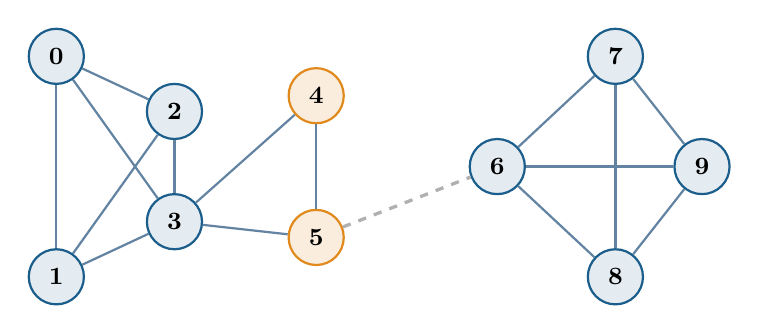
\begin{tikzpicture}[
    vtx/.style={circle, draw, thick, minimum size=7mm, inner sep=0pt,
      font=\small\bfseries},
    c3/.style={vtx, draw=core3, fill=core3!12},
    c1/.style={vtx, draw=core1, fill=core1!15},
    e/.style={thick, accent!70},
    br/.style={very thick, bridgecol, dashed}]
  % left K4
  \node[c3] (0) at (0,1.4) {0};
  \node[c3] (1) at (0,-1.4){1};
  \node[c3] (2) at (1.5,0.7){2};
  \node[c3] (3) at (1.5,-0.7){3};
  \foreach \a/\b in {0/1,0/2,0/3,1/2,1/3,2/3} \draw[e] (\a)--(\b);
  % triangle 3-4-5
  \node[c1] (4) at (3.3,0.9){4};
  \node[c1] (5) at (3.3,-0.9){5};
  \draw[e] (3)--(4); \draw[e] (3)--(5); \draw[e] (4)--(5);
  % bridge
  \node[c3] (6) at (5.6,0){6};
  \draw[br] (5)--(6);
  % right K4
  \node[c3] (7) at (7.1,1.4){7};
  \node[c3] (8) at (7.1,-1.4){8};
  \node[c3] (9) at (8.2,0){9};
  \foreach \a/\b in {6/7,6/8,6/9,7/8,7/9,8/9} \draw[e] (\a)--(\b);
\end{tikzpicture}
\caption{Spec Figure~1. \textcolor{core3}{$\blacksquare$}~$tc=3$
(each vertex is in a $K_4$); \textcolor{core1}{$\blacksquare$}~$tc=1$ (only in
$\{3,4,5\}$). The \textcolor{bridgecol}{dashed} bridge $(5,6)$ is in no triangle,
so it has level $0$ and never connects the two cores.}
\label{fig:g1}
\end{figure}

%======================================================================
\section{Computing $tc(v)$: Triangle-Core Peeling}
$tc(v)$ is obtained by a \textbf{peeling} (degeneracy) process on triangle
counts, exactly analogous to $k$-core decomposition:
\begin{enumerate}[leftmargin=1.6em, itemsep=2pt]
  \item Compute $t(v)=$ number of triangles containing $v$ in $G$.
  \item Repeatedly remove the vertex $v$ of \emph{smallest} current $t(v)$.
  Removing $v$ destroys every triangle through it, so for each such triangle
  $(v,a,b)$ decrement $t(a)$ and $t(b)$.
  \item $tc(v)$ is the value of $t(v)$ when $v$ is removed (the removal order
  keeps it monotone --- the ``max with running level'' rule).
\end{enumerate}
We keep vertices bucketed by current triangle count in the
\textbf{Batagelj--Zaversnik} array structure, so each removal and each triangle
destruction is $O(1)$; peeling is $O(n+T)$, where $T$ is the number of triangles.

\paragraph{Triangle enumeration.} Orient each edge from the lower- to the
higher-rank endpoint, $\mathrm{rank}=(d(\cdot),\,\mathrm{id})$. Intersecting
forward-neighbour lists then reports each triangle once, from its lowest-rank
vertex, in $\sum_{(u,w)\in E}\min\!\big(d(u),d(w)\big)=O(m^{1.5})$ time.

%======================================================================
\section{Index and Query}
\textsf{build()} stores two arrays:
\begin{itemize}[leftmargin=1.4em, itemsep=2pt]
  \item $tc[v]$ for every vertex --- $O(n)$;
  \item \texttt{level[\,]}, laid out \emph{parallel to}
  \texttt{graph.indices} (the flat adjacency array), so that a query is a plain
  threshold traversal --- $O(m)$.
\end{itemize}
$\textsf{query}(k,v)$ returns $[\,]$ if $tc(v)<k$; otherwise it runs a DFS from
$v$ that crosses only edges with $\texttt{level}\ge k$ (whose endpoints
then automatically satisfy $tc\ge k$) and returns the visited set.

\subsection{Worked Example (Figure~\ref{fig:g1})}
$tc=3$ on $\{0,1,2,3,6,7,8,9\}$ and $tc=1$ on $\{4,5\}$.
\begin{itemize}[leftmargin=1.4em, itemsep=2pt]
  \item $\textsf{query}(1,0)$: the $K_4$ edges and $(3,4),(3,5),(4,5)$ all have
  level $1$ (triangle $\{3,4,5\}$ has level $\min(3,1,1)=1$); the bridge $(5,6)$
  has level $0$. $\Rightarrow \{0,1,2,3,4,5\}$.
  \item $\textsf{query}(3,3)$: edges $(3,4),(3,5)$ have level $1<3$, so $4,5$ are
  excluded; only the $K_4$ edges (level $3$) are crossed.
  $\Rightarrow \{0,1,2,3\}$.
  \item $\textsf{query}(4,0)$: $tc(0)=3<4 \Rightarrow [\,]$.
\end{itemize}
\answer{$\textsf{query}(1,0)=\{0,1,2,3,4,5\}$,\quad
$\textsf{query}(3,3)=\{0,1,2,3\}$,\quad $\textsf{query}(4,0)=[\,]$.}

%======================================================================
\section{Correctness}
\begin{itemize}[leftmargin=1.4em, itemsep=3pt]
  \item \textbf{Peeling yields $tc$.} Identical to $k$-core correctness with
  ``triangle count'' as the monotone quantity: always removing the current
  minimum guarantees no later-removed vertex has a smaller core number, so each
  vertex's removal value equals $tc(v)$.
  \item \textbf{Edge level captures triangle connectivity.} If a triangle
  $(a,b,c)$ has $\min\big(tc(a),tc(b),tc(c)\big)\ge k$, then all three of its
  edges get level $\ge k$, making its vertices mutually reachable at level $k$;
  conversely an edge reaches level $k$ only through such a triangle. Chaining
  triangles that share a vertex therefore chains the DFS, so the reachable set is
  exactly the triangle-connected $k$-core component.
  \item \textbf{$v$ is always included.} $tc(v)\ge k$ means $v$ lies in a triangle
  of level $\ge k$, hence has an incident edge of level $\ge k$ and is reached.
\end{itemize}

%======================================================================
\section{Complexity Analysis}
Let $n$ be the number of vertices, $m$ the number of edges, $d(v)$ the degree of
$v$, $T$ the number of triangles ($T=O(m^{1.5})$), and $C$ the vertex set
returned by a query.

\subsection{Index construction time: $O\big(m^{1.5}+n\big)$}
\begin{center}
\begin{tabular}{@{}ll@{}}
\toprule
\textbf{Stage} & \textbf{Cost}\\
\midrule
Triangle listing (forward, degree-ordered) &
  $\displaystyle\sum_{(u,w)\in E}\min\!\big(d(u),d(w)\big)=O\big(m^{1.5}\big)$\\
Peeling (Batagelj--Zaversnik on triangle counts) & $O(n+T)$\\
Edge levels (aggregate $+$ scatter) & $O(T)+O(n+m)$\\
\midrule
\textbf{Total} & $O\big(m^{1.5}+n+m+T\big)=O\big(m^{1.5}+n\big)$\\
\bottomrule
\end{tabular}
\end{center}
since $T=O(m^{1.5})$ and $m=O(m^{1.5})$.

\subsection{Query time: $O\!\Big(\sum_{x\in C} d(x)+|C|\log|C|\Big)$}
A query is a single DFS over the induced subgraph of the answer, scanning each
returned vertex's adjacency once ($\sum_{x\in C}d(x)$), followed by an
$O(|C|\log|C|)$ sort that returns the vertices in canonical ascending order. Both
terms are \textbf{output-sensitive} --- bounded by the returned component --- and
the traversal term dominates in a genuine triangle core (every returned vertex
has degree $\ge 2$), so the query is effectively output-linear and $O(n+m)$ in
the worst case. The initial $tc(v)<k$ rejection is $O(1)$.

\subsection{Space: $O(n+m)$}
The persistent index is $tc[\,]$ ($O(n)$) plus \texttt{level[\,]} ($O(m)$),
so $O(n+m)$. Construction additionally uses $O(n+T)$ transient memory (the
triangle list and per-vertex triangle incidence), which may be released once
\textsf{build()} finishes.

%======================================================================
\section{Key Implementation Excerpt}
\begin{lstlisting}[style=py]
# --- peeling: tc(v) via Batagelj-Zaversnik buckets on triangle counts ---
for i in range(n):
    v = order[i]; lvl = d[v]; tc[v] = lvl            # smallest remaining count
    for t in tri_of[v]:                              # triangles through v
        if not alive[t]: continue
        alive[t] = 0                                 # triangle dies with v
        for w in triangles[t]:
            dw = d[w]
            if w == v or dw <= lvl: continue          # w already fixed, leave it
            p, s = pos[w], head[dw]                    # move w one bucket down
            f = order[s]
            if f != w:
                order[p], order[s] = f, w; pos[f], pos[w] = p, s
            head[dw] += 1; d[w] = dw - 1

# --- query: threshold DFS over edge levels ---
def query(self, k, v):
    if self.tc[v] < k: return []
    off, adj, level = self.graph.offsets, self.graph.indices, self.level
    seen = {v}; stack = [v]
    while stack:
        x = stack.pop()
        for i in range(off[x], off[x + 1]):
            if level[i] >= k and adj[i] not in seen:
                seen.add(adj[i]); stack.append(adj[i])
    return sorted(seen)          # canonical (ascending) vertex order
\end{lstlisting}

\end{document}
